%---------------------------------------------------------------------------------------------------
%
%	Edited by: Copyright (c) 2016 Jakub Kúdela
%   Based on: Copyright (c) 2015 Jan Küster
%
%	The MIT License (MIT)
%
%	Permission is hereby granted, free of charge, to any person obtaining a copy
%	of this software and associated documentation files (the "Software"), to deal
%	in the Software without restriction, including without limitation the rights
%	to use, copy, modify, merge, publish, distribute, sublicense, and/or sell
%	copies of the Software, and to permit persons to whom the Software is
%	furnished to do so, subject to the following conditions:
%	
%	THE SOFTWARE IS PROVIDED "AS IS", WITHOUT WARRANTY OF ANY KIND, EXPRESS OR
%	IMPLIED, INCLUDING BUT NOT LIMITED TO THE WARRANTIES OF MERCHANTABILITY,
%	FITNESS FOR A PARTICULAR PURPOSE AND NONINFRINGEMENT. IN NO EVENT SHALL THE
%	AUTHORS OR COPYRIGHT HOLDERS BE LIABLE FOR ANY CLAIM, DAMAGES OR OTHER
%	LIABILITY, WHETHER IN AN ACTION OF CONTRACT, TORT OR OTHERWISE, ARISING FROM,
%	OUT OF OR IN CONNECTION WITH THE SOFTWARE OR THE USE OR OTHER DEALINGS IN
%	THE SOFTWARE.
%
%---------------------------------------------------------------------------------------------------


%===================================================================================================
%	DOCUMENT DEFINITION
%===================================================================================================

%we use article class because we want to fully customize the page and dont use a cv template
\documentclass[10pt,a4paper]{article}	

%---------------------------------------------------------------------------------------------------
%	ENCODING
%---------------------------------------------------------------------------------------------------

%we use utf8 since we want to build from any machine
\usepackage[utf8]{inputenc}		
\usepackage{fontawesome}
%---------------------------------------------------------------------------------------------------
%	LOGIC
%---------------------------------------------------------------------------------------------------

% provides \isempty test
\usepackage{xifthen}

%---------------------------------------------------------------------------------------------------
%	FONT
%---------------------------------------------------------------------------------------------------

% some tex-live fonts - choose your own

%\usepackage[defaultsans]{droidsans}
%\usepackage[default]{comfortaa}
%\usepackage{cmbright}
\usepackage[default]{raleway}
%\usepackage{fetamont}
%\usepackage[default]{gillius}
%\usepackage[light,math]{iwona}
%\usepackage[thin]{roboto}
\usepackage{hyperref}

% set font default
\renewcommand*\familydefault{\sfdefault} 	
\usepackage[T1]{fontenc}

% more font size definitions
\usepackage{moresize}		

%---------------------------------------------------------------------------------------------------
%	PAGE LAYOUT  DEFINITIONS
%---------------------------------------------------------------------------------------------------

%debug page outer frames
%\usepackage{showframe}			

%define page styles using geometry
\usepackage[a4paper]{geometry}		

% for example, change the margins to 2 inches all round
\geometry{top=1.75cm, bottom=-.6cm, left=1.5cm, right=1.5cm} 	

%use customized header
\usepackage{fancyhdr}		
\pagestyle{fancy}

%less space between header and content
\setlength{\headheight}{-5pt}		

%customize entries left, center and right
\lhead{}
\chead{\small{
  Guowei Lu $\cdot$ 
  Delft, The Netherlands $\cdot$ 
  \textcolor{sectcol}{\textbf{\href
  {https://pasu.github.io}
  {\faHome}}} $\cdot$ 
  \textcolor{sectcol}{\textbf{\href
  {mailto:g.lu-1@tudelft.nl}
  {\faEnvelope }}}
}}
\rhead{}

%indentation is zero
\setlength{\parindent}{0mm}

%---------------------------------------------------------------------------------------------------
%	TABLE /ARRAY DEFINITIONS
%--------------------------------------------------------------------------------------------------- 

%for layouting tables
\usepackage{multicol}			
\usepackage{multirow}

%extended aligning of tabular cells
\usepackage{array}
\newcolumntype{x}[1]{>{\raggedleft\hspace{0pt}}p{#1}}

%---------------------------------------------------------------------------------------------------
%	GRAPHICS DEFINITIONS
%--------------------------------------------------------------------------------------------------- 

%for header image
\usepackage{graphicx}

%for floating figures
\usepackage{wrapfig}
\usepackage{float}
%\floatstyle{boxed} 
%\restylefloat{figure}

%for drawing graphics		
\usepackage{tikz}				
\usetikzlibrary{shapes, backgrounds,mindmap, trees}

%---------------------------------------------------------------------------------------------------
%	Color DEFINITIONS
%--------------------------------------------------------------------------------------------------- 

\usepackage{color}

%accent color
\definecolor{sectcol}{RGB}{90,90,120}

%dark background color
\definecolor{bgcol}{RGB}{110,110,110}

%light background / accent color
\definecolor{softcol}{RGB}{225,225,225}

%===================================================================================================
%	DEFINITIONS
%===================================================================================================

%---------------------------------------------------------------------------------------------------
% 	HEADER
%---------------------------------------------------------------------------------------------------

% remove top header line
\renewcommand{\headrulewidth}{0pt} 

%remove botttom header line
\renewcommand{\footrulewidth}{0pt}	  	

%remove pagenum
\renewcommand{\thepage}{}	

%remove section num		
\renewcommand{\thesection}{}			

%---------------------------------------------------------------------------------------------------
% 	ARROW GRAPHICS in Tikz
%---------------------------------------------------------------------------------------------------

% a six pointed arrow poiting to the left
\newcommand{\tzlarrow}{(0,0) -- (0.2,0) -- (0.3,0.2) -- (0.2,0.4) -- (0,0.4) -- (0.1,0.2) -- cycle;}	

% include the left arrow into a tikz picture
% param1: fill color
%
\newcommand{\larrow}[1]{
  \begin{tikzpicture}[scale=0.58]
    \filldraw[fill=#1!100,draw=#1!100!black]  \tzlarrow
  \end{tikzpicture}
}

% a six pointed arrow poiting to the right
\newcommand{\tzrarrow}{ (0,0.2) -- (0.1,0) -- (0.3,0) -- (0.2,0.2) -- (0.3,0.4) -- (0.1,0.4) -- cycle;}

% include the right arrow into a tikz picture
% param1: fill color
%
\newcommand{\rarrow}{
  
\begin{tikzpicture}[scale=0.7]
    \filldraw[fill=sectcol!100,draw=sectcol!100!black] \tzrarrow
  \end{tikzpicture}
}
%---------------------------------------------------------------------------------------------------
%	custom sections
%---------------------------------------------------------------------------------------------------

% create a coloured box with arrow and title as cv section headline
% param 1: section title
%
\newcommand{\cvsection}[1]{
  \vspace{10pt}
  \colorbox{sectcol}{\mystrut \makebox[1\linewidth][l]{
    \larrow{bgcol} \hspace{-8pt} \larrow{bgcol} \hspace{-8pt} 
    \larrow{bgcol}\textcolor{white}{\textbf{#1}}\hspace{4pt}
  }}\\
}

%create a coloured arrow with title as cv meta section section
% param 1: meta section title
%
\newcommand{\metasection}[2]{
  \begin{tabular*}{1\textwidth}{p{2.4cm} p{11cm}}
    \larrow{bgcol} \normalsize{\textcolor{sectcol}{#1}}&#2\\[10pt]
  \end{tabular*}
}

\newenvironment{onecolentry}{
    \begin{adjustwidth}{
        0.2 cm + 0.00001 cm
    }{
        0.2 cm + 0.00001 cm
    }
}{
    \end{adjustwidth}
} % new environment for one column entries

\newenvironment{twocolentry}[2][]{
    \onecolentry
    \def\secondColumn{#2}
    \setcolumnwidth{\fill, 4.5 cm}
    \begin{paracol}{2}
}{
    \switchcolumn \raggedleft \secondColumn
    \end{paracol}
    \endonecolentry
} % new environment for two column entries

%---------------------------------------------------------------------------------------------------
%	 CV EVENT
%---------------------------------------------------------------------------------------------------

% creates a stretched box as cv entry headline followed by two paragraphs
% param 1:	event time i.e. 2014 or 2011-2014 etc.
% param 2:	event name (what did you do?)
% param 3:	institution (where did you work / study)
%
\newcommand{\cvevent}[3]{
  \begin{tabular*}{1\textwidth}{p{2.5cm} p{10.5cm} x {4.0cm}}
    \textcolor{bgcol}{#1} & \textbf{#2} & \vspace{2.5pt}\textcolor{sectcol}{#3}
  \end{tabular*}
  \vspace{-10pt}
  \textcolor{softcol}{\hrule}
  \vspace{10pt}
}

% creates a stretched box as cv entry detail 
% param 1:	information describing the event
%
\newcommand{\cvdetail}[1]{
  \begin{tabular*}{1\textwidth}{p{2.5cm} p{14.5cm}}
    & \larrow{bgcol}  #1\\ [3pt]
  \end{tabular*}
}

\newcommand{\pubdetail}[1]{
  \begin{tabular*}{1\textwidth}{p{2.5cm} p{14.5cm}}
    & #1\\ [3pt]
  \end{tabular*}
}

%---------------------------------------------------------------------------------------------------
% CUSTOM STRUT FOR EMPTY BOXES
%---------------------------------------------------------------------------------------------------
\newcommand{\mystrut}{\rule[-.3\baselineskip]{0pt}{\baselineskip}}

%===================================================================================================
%	DOCUMENT CONTENT
%===================================================================================================
\title{resume}
\begin{document}

% use our custom fancy header definitions
\pagestyle{fancy}	

%---------------------------------------------------------------------------------------------------
%	TITLE HEADLINE
%---------------------------------------------------------------------------------------------------

\vspace{-20pt}

% use this for single words, e.g. CV or RESUME etc.
\hspace{-0.25\linewidth}\colorbox{bgcol}{
  \makebox[1.5\linewidth][c]{
    \HUGE{\textcolor{white}{\textsc{Peter Lu}}} 
    \textcolor{sectcol}{\rule[-1mm]{1mm}{0.9cm}} 
    \HUGE{\textcolor{white}{\textsc{Resume}}}
  }
}

%---------------------------------------------------------------------------------------------------
%	HEADER IMAGE
%---------------------------------------------------------------------------------------------------

\begin{figure}[H]
\begin{flushright}
  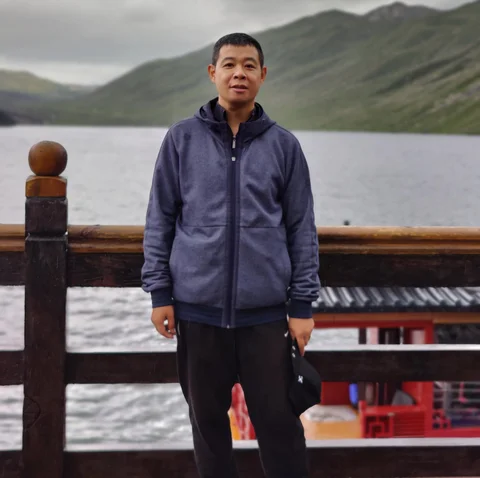
\includegraphics[width=0.2\linewidth]{prof_pic-480.png}
\end{flushright}
\end{figure}

%---------------------------------------------------------------------------------------------------
%	META SECTION
%---------------------------------------------------------------------------------------------------

\vspace{-115pt}

\metasection{Status:}{PhD candidate in Computer Graphics}
\metasection{Skills:}{C++, JS, Python, WebGL/OpenGL, CUDA} 
\metasection{Interests:}{Rendering, 3D GIS}
\metasection{Activities:}{Running, writing, music}

%---------------------------------------------------------------------------------------------------
%	SUMMARAY (optional)
%---------------------------------------------------------------------------------------------------

\cvsection{Summary}

I am a PhD candidate in the Computer Graphics and Visualization (CGV) group at TU Delft, working under the supervision of Dr. Petr Kellnhofer and Prof. Elmar Eisemann. My research specializes in virtual reality rendering, with a focus on realistic material representations and advanced lighting models. I also have a strong interest in offline and differentiable rendering techniques.

During my studies, I gained industry experience as a 3D GIS engineer at SuperMap, where I worked on projects involving virtual earth systems and advanced mapping solutions.

%===================================================================================================
%	CV SECTIONS AND EVENTS (MAIN CONTENT)
%===================================================================================================

%---------------------------------------------------------------------------------------------------
%	EDUCATION SECTION
%---------------------------------------------------------------------------------------------------
\cvsection{Education}

\cvevent{'22/06 - now}{PhD candidate}{TU Delft}
\cvdetail{\textbf{VR Renovate Project}: The VR Renovate project focuses on developing real-time graphics and VR technology to visually showcase the results of sustainable home renovations.}
\cvdetail{\textbf{Teachers Assistant}: Applied Image Processing, 3D Visualization.}

\cvevent{2018 - 2020}{Master's Degree, Computer Science}{Utrecht University}
\cvdetail{\textbf{Courses}: Advanced Graphics, Optimization and Vectorization, Game Physics, Computer Vision, Geometric Algorithm,
Motion and Manipulation, Crowd Simulation etc.}
\cvdetail{\textbf{Master Thesis}: ‘Gradient-Domain Volume Rendering’}
\cvdetail{\textbf{GPA}: 8.73/10 (Cum Laude)}


\cvevent{2002 - 2006}{Bachelor's Degree, Information System}{Beijing Forestry University}

%---------------------------------------------------------------------------------------------------
%	EXPERIENCE
%---------------------------------------------------------------------------------------------------
\cvsection{EXPERIENCE}

\cvevent{2006 - 2022}{Technical Leader/Engineer, R\&D Department}{SuperMap}
\cvdetail{\textbf{3D GIS}: I work on real-time rendering and WebGL, handling 3D models like terrain and BIM, improving visual quality, and optimizing performance. My tasks include LOD scheduling, rendering effects, and GPU/CPU optimization.}
\cvdetail{\textbf{Map Module}: I developed the map module, focusing on styled vector maps, text rendering, anti-aliasing, and cross-platform compatibility across Windows, Linux, Android, and Unix.}

%---------------------------------------------------------------------------------------------------
%	Publications
%---------------------------------------------------------------------------------------------------
\cvsection{PUBLICATIONS}

\begin{itemize}
\item \textbf{Guowei Lu}, Jerry Guo, Petr Kellnhofer, Elmar Eisemann. \href{https://dl.acm.org/doi/10.1145/3670947.3670952}{Sheared Polygonal Texture Filtering}. Best student paper in \textit{Graphics Interface}, 2024.
\item \textbf{Guowei Lu}. Gradient-Domain Volume Rendering. Master Thesis at \textit{Utrecht University}, 2020.
\end{itemize}

%---------------------------------------------------------------------------------------------------
%	Publications
%---------------------------------------------------------------------------------------------------
\cvsection{PROJECTS}

\cvevent{2017}{\href{https://github.com/pasu/ExamplesforCesium}{ExamplesforCesium}}{JS, WebGL}
\cvdetail{tutorials for Cesium and a gallery showcasing various Cesium demos.}

*\textit{For all projects, please visit my \href{https://pasu.github.io/CV/project_portfolio.html}{project portfolio}.}

%===================================================================================================
%	DOCUMENT END
%===================================================================================================
\end{document}
